\scanpage{23}
\mspage{3}
admet une description purement algébrique, valable \inserted{pour des schémas lisses} sur un corps \deleted{de car} quelconque.
Elle est \uline{filtrée}, le \unsure{gradué} associé étant les termes $E_\infty$ associé à une suite spectrale (*). Voir pour des commentaires mes papiers bleus$\ldots$

5) \uline{Critique du point de vue : Cohomologie de De Rham}.

\deleted{a) \unsure{Il ne reste plus (comme pour)} \unsure{toute l'étude de la} \unsure{K-théorie et théorie des classes de cohomologie} \unsure{associées} à des cycles (cf. \unsure{Pb des classes alg. de Hodge}, dans \unsure{mon récent exp. Bourb.})}

\margin{\figure{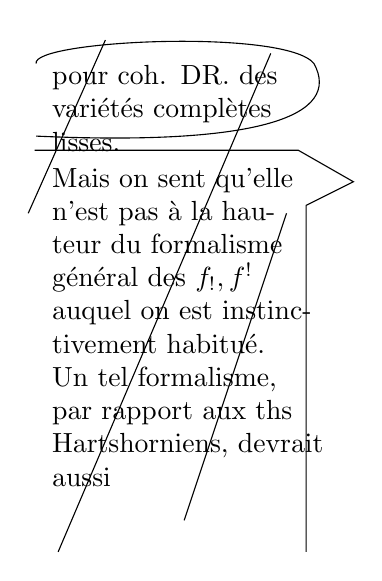
\begin{tikzpicture}[x=1cm,y=1cm]
\node[align=left,text width=3.4cm,anchor=north west] at (0,0) {\deleted{pour coh. DR. des variétés complètes \unsure{lisses}.}};
\draw (-.08,-.10) .. controls (-.15,.2) and (3.1,.35) .. (3.45,-.1) .. controls (3.8,-.75) and (2.8,-1.15) .. (-.08,-1.02);
\node[align=left,text width=3.5cm,anchor=north west] at (0,-1.3) {\deleted{Mais on sent qu'elle n'est pas à la hauteur du formalisme général des $\unsure{f_!,f^!}$ auquel on est \unsure{instinctivement} habitué. Un tel formalisme, \unsure{par rapport aux ths Hartshorniens}, devrait \unsure{aussi}}};
\draw (-.1,-1.2)--(3.25,-1.2)--(3.95,-1.6)--(3.35,-1.9)--(3.35,-6.3);
\draw (.8,.2)--(-.18,-2.0);
\draw (2.9,.03)--(.2,-6.3);
\draw (3.1,-2.0)--(1.8,-5.9);
\end{tikzpicture}}}

\deleted{\unsure{b)}} En car. $\unsure{0}$, pour \unsure{les variétés non singulières}, on trouve des invariants excellents, donnant en particulier les ``bons'' nombres de Betti.
Mais en car $p$, c'est moins raisonnable, car
1°) Si $X$ n'est pas propre, on trouve en général des vectoriels de dim infinie
\[
\unsure{\text{p. ex.}|\text{Ex.}}\qquad H_{\mathrm{DR}}^0(X)\simeq H^0(X,\underline O_X)^p\ ;
\]
2°) Même si $X$ est propre, on ne trouve pas en général les ``bons'' nombres de Betti ; par exemple on a
\[
\dim H_{\mathrm{DR}}^1(X)\ \deleted{\unsure{=}}\geq 2\dim\underline{\mathrm{Pic}}_X,
\]
et il y a des exemples où on a $>$, (dû vraisemblablement à des phénomènes de $p$-torsion $\ldots$).

Enfin 3°) Même dans des cas (tels celui des VA) où les $\dim H_{\mathrm{DR}}^i(X)\deleted{\unsure{=b^i(X)}}$ sont les ``bons'' $b^i(X)$, un défaut majeur de ces \unsure{esp. v.} (déjà signalé par Serre) c'est que le corps de
\margin{22}
